\subsection*{Teil B: Lineare Funktionen (35 Minuten)}

\begin{enumerate}[label=\arabic*.,resume]

    \item \textbf{Proportionale Funktionen ($f(x) = mx$):}

    \begin{enumerate}[label=\alph*)]
        \item Welche Funktion gehört zu welchem Graph? Ordne zu:

        \begin{center}
            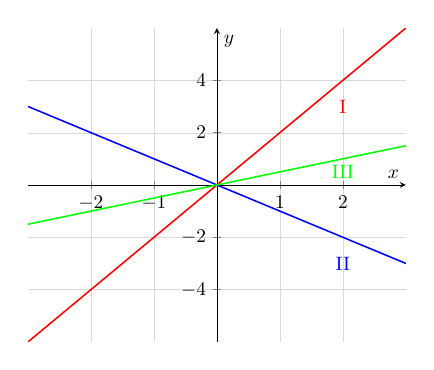
\begin{tikzpicture}[scale=0.7]
                \begin{axis}[
                    axis lines = center,
                    xlabel = $x$,
                    ylabel = $y$,
                    xmin=-3, xmax=3,
                    ymin=-6, ymax=6,
                    xtick={-2,-1,0,1,2},
                    ytick={-4,-2,0,2,4},
                    grid=major,
                    grid style={line width=0.1pt,draw=gray!30},
                ]
                    \addplot[thick, red, domain=-3:3] {2*x};
                    \addplot[thick, blue, domain=-3:3] {-x};
                    \addplot[thick, green, domain=-3:3] {0.5*x};
                    \node[red] at (axis cs:2,3) {I};
                    \node[blue] at (axis cs:2,-3) {II};
                    \node[green] at (axis cs:2,0.5) {III};
                \end{axis}
            \end{tikzpicture}
        \end{center}

        Graph I: $f(x) = $ \underline{\hspace{3cm}} \hspace{1cm}
        Graph II: $f(x) = $ \underline{\hspace{3cm}} \hspace{1cm}
        Graph III: $f(x) = $ \underline{\hspace{3cm}}

        \item Zeichne den Graphen von $f(x) = -3x$:

        \begin{center}
            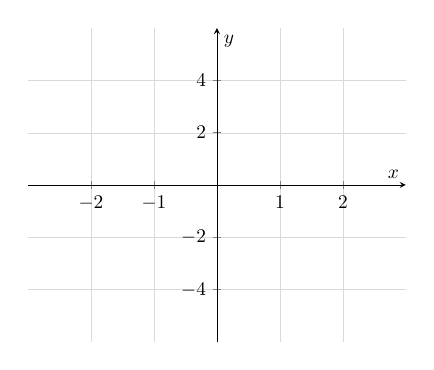
\begin{tikzpicture}[scale=0.7]
                \begin{axis}[
                    axis lines = center,
                    xlabel = $x$,
                    ylabel = $y$,
                    xmin=-3, xmax=3,
                    ymin=-6, ymax=6,
                    xtick={-2,-1,0,1,2},
                    ytick={-4,-2,0,2,4},
                    grid=major,
                    grid style={line width=0.1pt,draw=gray!30},
                ]
                \end{axis}
            \end{tikzpicture}
        \end{center}

    \end{enumerate}

    \item \textbf{Allgemeine lineare Funktionen ($f(x) = mx + t$):}

    \begin{enumerate}[label=\alph*)]
        \item Bestimme Steigung $m$ und y-Achsenabschnitt $t$:

        \textit{Beispiel:} $f(x) = 4x - 3$ \hspace{2cm} $m = 4$, $t = -3$

        \vspace{0.5cm}
        \begin{tabular}{ll}
            $f(x) = 2x + 5$ & $m = $ \underline{\hspace{2cm}}, $t = $ \underline{\hspace{2cm}} \\[1ex]
            $f(x) = -3x + 7$ & $m = $ \underline{\hspace{2cm}}, $t = $ \underline{\hspace{2cm}} \\[1ex]
            $f(x) = 0,5x - 2$ & $m = $ \underline{\hspace{2cm}}, $t = $ \underline{\hspace{2cm}} \\[1ex]
            $f(x) = -x + 4$ & $m = $ \underline{\hspace{2cm}}, $t = $ \underline{\hspace{2cm}}
        \end{tabular}

        \vspace{1cm}

        \item Funktionsgleichung aus zwei Punkten bestimmen:

        Gegeben: A(1|3) und B(3|7)

        Steigung: $m = \frac{y_2 - y_1}{x_2 - x_1} = \frac{7-3}{3-1} = $ \underline{\hspace{3cm}}

        Mit A(1|3): $3 = $ \underline{\hspace{2cm}} $ \cdot 1 + t$ \hspace{1cm} $\Rightarrow t = $ \underline{\hspace{3cm}}

        Funktionsgleichung: $f(x) = $ \underline{\hspace{6cm}}

    \end{enumerate}

    \item \textbf{Nullstelle berechnen:}

    Bei der Nullstelle ist $f(x) = 0$. Berechne die Nullstelle von $f(x) = 2x - 8$:

    \vspace{2.5cm}

    Nullstelle: $x_0 = $ \underline{\hspace{4cm}}

\end{enumerate}